% % % % % % % % % % % % % % % % % % % % % % % % % % % % % % % % % % % % % % % % 
% Formelsammlung von LaTeX4EI									
%
% @encode: 	UTF-8, tabwidth = 4, newline = LF
% @author:	Emanuel Regnath
% @date:		
%
% % % % % % % % % % % % % % % % % % % % % % % % % % % % % % % % % % % % % % % % 

%---------------------------------------%
%		Elektromagn. Verträglichkeit	%
%~~~~~~~~~~~~~~~~~~~~~~~~~~~~~~~~~~~~~~~%

% Document Class ===============================================================
\documentclass[fs, footer]{latex4ei}

\setlength{\tabcolsep}{0.4em}
\usepackage{layout}


% DOCUMENT_BEGIN ===============================================================
\begin{document}



% Split in 4 Columns ===========================================================
\begin{multicols*}{4}

% TITLE ========================================================================
\fstitle{Elektromagnetische \\ Verträglichkeit}



% SECTION ====================================================================================
\section{Einführung}
% ============================================================================================
\sectionbox{
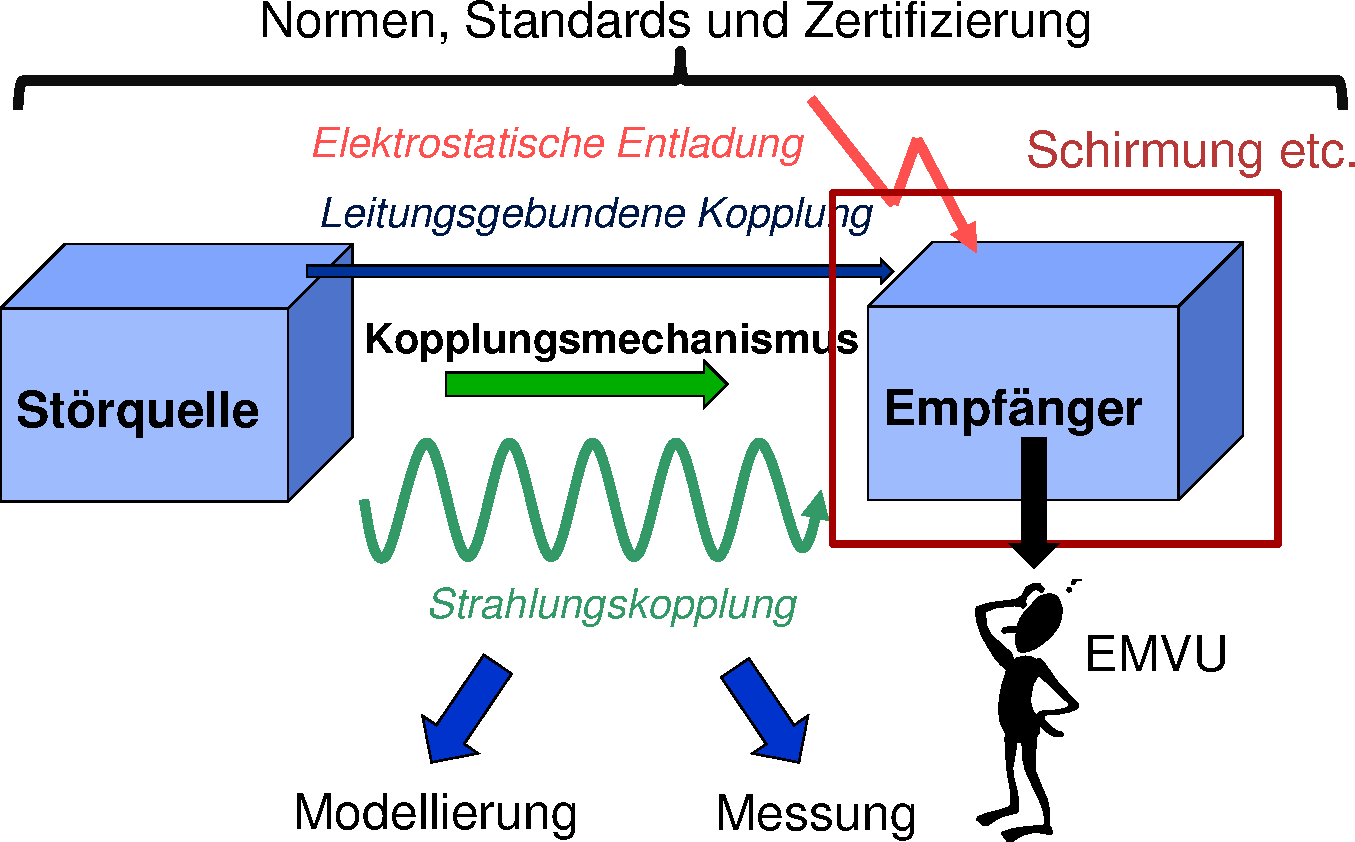
\includegraphics[width = \columnwidth]{./img/EMV.pdf}}


	%AM: Amplitude Modulation \qquad FM: requency Modulation\\
	%Impulsbandbreite: $H(f)$ \qquad Rauschbandbreite: $H^2(f)$\\
	%IS: Impulse Area $IS = A \cdot t$\\

%Leistungspegel: $L = 10 \lg \frac{P}{P_0} \si{\decibel} = 10 \lg \frac{A^2}{A_0^2} \si{\decibel} = 20 \lg \frac{A}{A_0} \si{\decibel}$ 


\sectionbox{
	


	\subsection{Frequenzanalyse}
	\begin{tabular}{ll}
		Zeitbereich & Frequenzbereich\\ \mrule
		Harmonische Schwingung & Schmalbandig(Impuls)\\
		schmalbandig(Impuls) & Breitbandig\\
		Eckig, kantig & Hohe Frequenzen\\
		Rauschen & Rauschen\\
	\end{tabular}


	\subsection{Frequenztabelle}
	\begin{tabular}{@{}llll} 			%Frequenz, Energie, Wellenlänge, Anwendung
		$\SI{50}{\hertz}$ & Stromnetz & $\SI{1}{\peta\hertz}$ & UV-Strahlung\\
		$\SI{2.45}{\giga\hertz}$ & Mikrowelle, WLAN & $\SI{1}{\exa\hertz}$ & Röntgenstrahlung\\	
		$\SI{600}{\tera\hertz}$ & Sicht. Licht & $\SI{30}{\exa\hertz}$ & Radioaktiv\\
	\end{tabular}
}

% SECTION ====================================================================================
\section{Normen und Standards}
% ============================================================================================
\sectionbox{
Arten: Gesetzliche, Militärische und Medizinische Standards.\\
Geregelt werden Grenzwerte sowie Mess- und Prüfmethoden.\\
	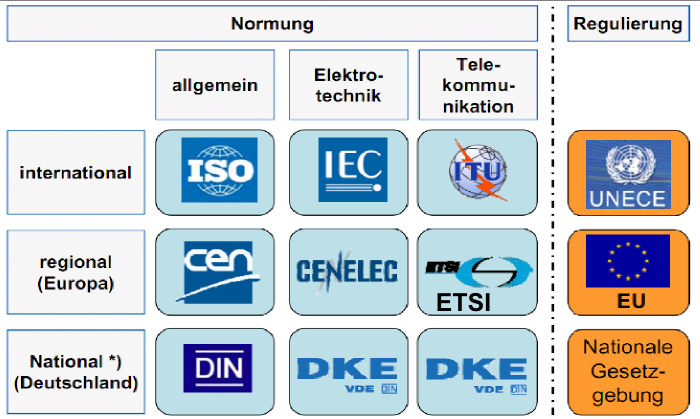
\includegraphics[width = \columnwidth]{./img/normen.png}
	Ratgeber: ANSI/IEEE \qquad Dauer bis gültige Norm: $\approx$ 5 Jahre\\
	Zertifikate: TÜV GS: Geprüfte Sicherheit; CE: Kein Gütesiegel\\
	Frequenznutzungsplan von $\SI{9}{\kilo \hertz}$ bis $\SI{275}{\giga \hertz}$: Bundesnetzagentur\\
	ISO: International Organization for Standardization\\
	IEC: International Electrical Commission\\
	ITU: International Telecommunication Union\\
	DKE: Deutsche Kommission Elektrotechnik
}

\sectionbox{
	\subsection{Spezifische Absorptionsrate SAR}
	$\mathrm{SAR} = \frac{j^2}{\rho \sigma} = $ \qquad $\unitof{\mathrm{SAR}} = \si{\watt \per \kilogram}$\\ 
	Europa: 2 \qquad USA: 1.6 \qquad China: $< 1$
}
	
	
	


% SECTION ====================================================================================
\section{Quellen der EMB}
% ============================================================================================

\sectionbox{
	\subsection{Störquellen}
	Systeme: Mobilfunk, Radar, GPS, RFID, Hochspannungsleitungen\\
	Schaltungen: Autozündung, Schalter, Motoren, Lautsprecher \\
	Natürlich: Blitze, Hintergrundstrahlung, Sonnenwinde\\
	Nichtlineare Bauteile erzeugen Oberschwingungen.\\


	\subsection{Blitze}
	Ein Blitz ist ein Plasma, welches aus Ionen, Elektronen und Neutralteilchen besteht. 
	90\% der Entladungen finden zwischen den Wolken statt.\\
	Stromfluss $\SI{200}{\kilo\ampere}$ \qquad El. Feld: $1 - \SI{10}{\kilo\volt\per\meter}$\\ 
	Donner: Luft erwärmt sich so schnell, dass sie sich mit Überschall ausdehnt.
}

% SECTION ====================================================================================
\section{Kopplung}
% ============================================================================================

\sectionbox{
	\begin{tabular}{l@{\hspace{2em}}l} \trule
	{\large Objekt $\ll$ Wellenlänge} & {\large Objekt $\approx$ Wellenlänge}\\
	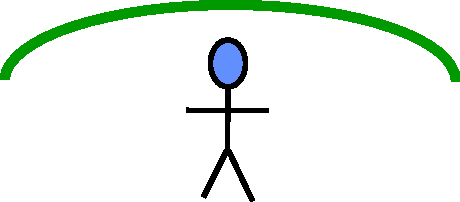
\includegraphics[width = 3cm]{./img/wave_larger.pdf} & 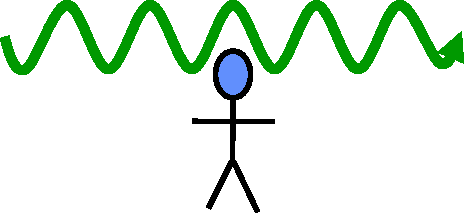
\includegraphics[width = 3cm]{./img/wave_equal.pdf}\\ \mrule
	\textbf{Galvanische Kopplung} & \textbf{Elektromagnetische Kopplung}\\
	\textbf{Kapazitive Kopplung} & \textbf{Leitungskopplung}\\
	\textbf{Induktive Kopplung} & \textbf{Strahlungskopplung}\\ \brule
	\end{tabular}
}

\sectionbox{
	\subsection{Objekt $\ll$ Wellenlägen}
	
	\subsubsection{Galvanische Kopplung}
	Transferimpedanz $\cx Z_T$
	
	\subsubsection{Kapazitive Kopplung}
	Verringerung des Leiterabstandes im System\\
	Vergrößerung des Abstandes zwischen den Systemen\\
	Einseitige Erdung bei niedrigen Frequenzen, beidseitig bei Hohen\\

	\subsubsection{Induktive Kopplung}
	Verringerung des Leiterabstandes im System\\
	Vergrößerung des Abstandes zwischen den Systemen\\
	Schirmung, Verdrillen, Senkrechte Anordnung
}
\sectionbox{
	\subsection{Objekt $\approx$ Wellenlänge}

		\subsubsection{Elektromagnetische Kopplung}
	
		\subsubsection{Leitungskopplung} 
		Reflexionskoeffizient $\Gamma = \frac{\norm{\vec E^-_{\ir Ref}}}{\norm{\vec E^+_{\ir In}}} = \frac{Z_{\ir new} - Z_0}{Z_{\ir new} + Z_0}$
	
	
		Hin- und Rücklaufende Welle: $\cx U(z) = \cx U^+ e^{-\Gamma z} + U^- e^{\Gamma z} = \frac12(U_0 + \cx Z I_0)e^{-\Gamma z} + \frac12 (U_0 - \cx Z I_0) e^{\Gamma z}  $\\
		Offene Leitung: Reflexionsfrei, konstanter Widerstand\\
		Abgeschlossene Leitung: Reflexionen, veränderlicher Widerstand\\
		Stehwellenverhältnis (VSWR): $s = \frac{V_{\max}}{V_{\min}} = \frac{I_{\max}}{I_{\min}}$\\
}

\sectionbox{
		\subsubsection{Strahlungskopplung}
		Fernfeld: $\vec k \vec r = \frac{2\pi r}{\lambda} \gg 1$ \qquad Nahfeld: $\vec k \vec r = \frac{2\pi r}{\lambda} \ll 1$\\

		\begin{tabular}{l@{\hspace{1cm}}l}
			\textbf{Elektrischer Dipol:} Stab & \textbf{Magnetischer Dipol:} Ring\\ \mrule

			\begin{tabular}{cccc}
					& $\frac{1}{r}$ & $\frac{1}{r^2}$ & $\frac{1}{r^3}$\\ \mrule
				$E_r$ & $-$ & \checkmark & \checkmark\\
				$E_\varphi$ & \checkmark & \checkmark & \checkmark\\
				$H_r$ & $-$ & $-$ & $-$\\
				$H_\theta$ & \checkmark & \checkmark & $-$\\
			\end{tabular}
			&
			\begin{tabular}{cccc}
					& $\frac{1}{r}$ & $\frac{1}{r^2}$ & $\frac{1}{r^3}$\\ \mrule
				$E_r$ & $-$ & $-$ & $-$\\	
				$E_\varphi$ & \checkmark & \checkmark & $-$\\
				$H_r$ & $-$ & \checkmark & \checkmark\\
				$H_\theta$ & \checkmark & \checkmark & \checkmark\\
			\end{tabular}
		\end{tabular}


		Greensche Funktion $G(\vec r, \vec r')$: Impulsantwort des freien Raums für eine Punktladung
}

		

		

\sectionbox{
	\subsection{Leitungsbeläge}
	Elektrostatik (NF): $R', G', C', L'$ \qquad Elektrodynamik (HF): $\gamma, \cx Z$\\

	\begin{tabular}{@{}lcccc@{}} \trule
	 & Koaxial & Doppel & Einzel & Parallel\\ 
	 & 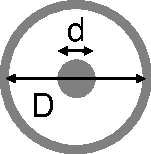
\includegraphics[scale = 0.3]{./img/koaxial.pdf} & 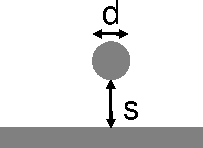
\includegraphics[scale = 0.3]{./img/einzel.pdf} & 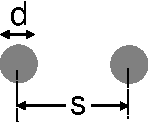
\includegraphics[scale = 0.3]{./img/doppel.pdf} & 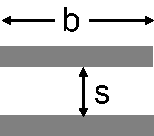
\includegraphics[scale = 0.3]{./img/parallel.pdf}\\ \mrule
	$R'$ & $\frac{R_A}{\pi} \left( \frac{1}{d} + \frac{1}{D} \right)$ & $\frac{R_A}{\pi d} \frac{2 s}{\sqrt{s^2 -d^2}}$ & $\frac{R_A}{\pi d} \frac{2 s}{\sqrt{4s^2 -d^2}}$ & $\frac{2 R_A}{b}$\\[1.5em]
	$C'$ & $\frac{2 \pi \varepsilon}{\ln \frac{D}{d} }$ & $\frac{\pi \varepsilon}{\arccos\left( \frac{s}{d} \right)}$ & $\frac{2 \pi \varepsilon}{\arccos\left( \frac{2 s}{d} \right)}$ & $\frac{\varepsilon b}{s}$\\[1.5em]
	$L'$ & $\frac{\mu}{2 \pi} \ln \frac{D}{d} $ & $\frac{\mu}{\pi} \arccos\left( \frac{s}{d} \right)$ & $\frac{\mu}{2 \pi} \arccos\left( \frac{2 s}{d} \right)$ & $\frac{\mu s}{b}$\\ \brule
	\end{tabular}
}

\sectionbox{
	\subsection{Leitungsgleichung \qquad LGS mit $\vec U, \vec I \in \C^n$}
	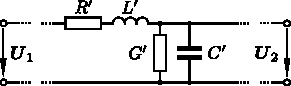
\includegraphics{./img/Leitung2.pdf}\\
	
	System DGLs: $\dot{\vec U}(x) = -\i \omega \ma L \vec I(x)$ \qquad $\dot{\vec I}(x) = -\i \omega \ma C \vec U(x)$\\
	$\vect{\vec U(l) \\ \vec I(l)} = \mat{\cos(\beta l) \ma E_n & -\i \omega \frac{\sin(\beta l)}{\beta} \ma L \\ -\i \omega \frac{\sin(\beta l)}{\beta} \ma C & \cos(\beta l) \ma E_n } \vect{\vec U(0) \\ \vec I(0)}$\\

	Bei Einspeisung von Strom/Spannung in Leitung 1 kann eingekoppelter Strom/Spannung in Leitung $n$ analytisch berechnet werden.
}

% SECTION ====================================================================================
\section{Messungen}
% ============================================================================================
EMI: Emissionsmessung \qquad EMS: Störfestigkeitsmessung 
\sectionbox{
	\subsection{Messkammer}
	Reflexionsarme Wände (Absorber), Gitterboden unter dem die Kabel verlaufen. Messequipment außerhalb der Kammer. Keine Fenster, nur Kamera\\
	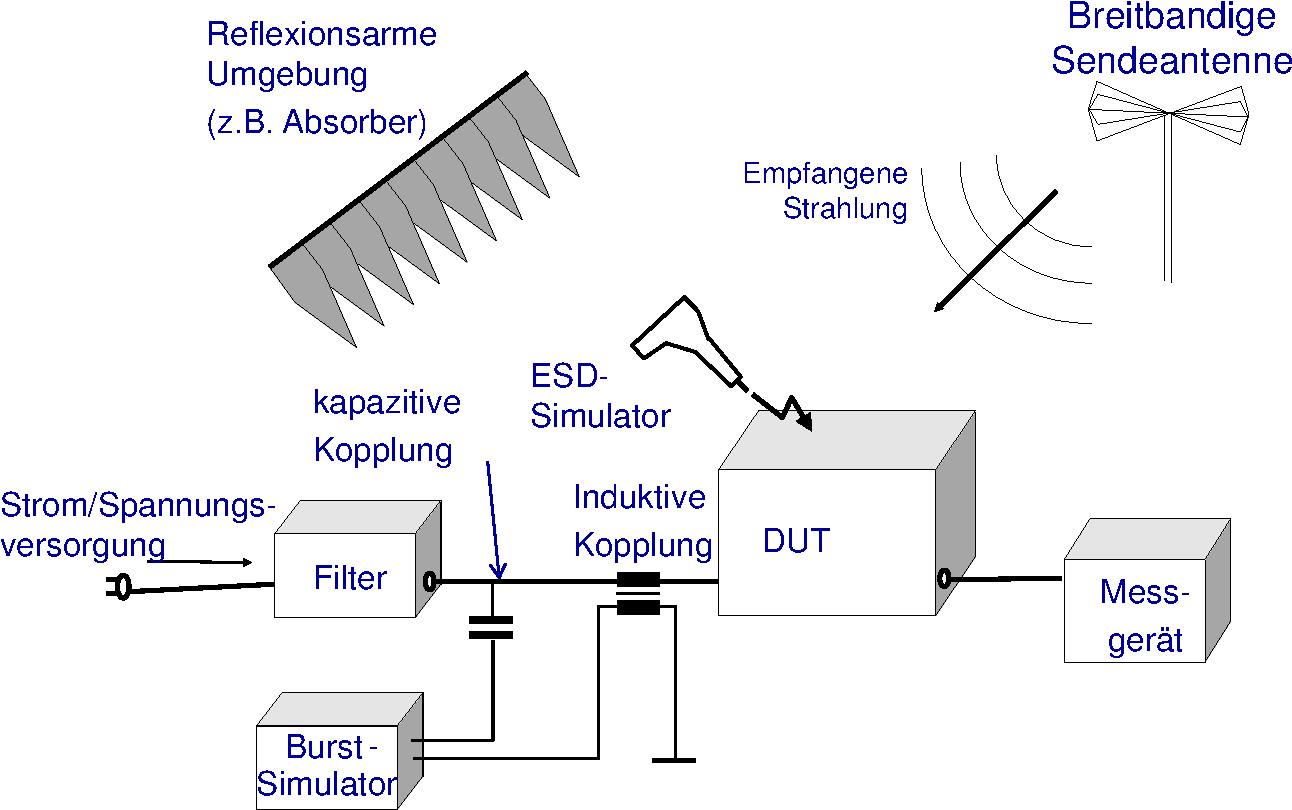
\includegraphics[width = \columnwidth]{./img/messung.pdf}
	\begin{description}
		\item[Antenne:] Breitbandige drehbare Antenne
		\item[Kabel:] Kabel müssen in kleinen Schleifen verkürzt werden und nicht zu Rollen gewickelt werden
		\item[Absorber:] Graphitgetränkte Pyramidenabsorber: Teil der Welle dringt ein der andere Teil wird reflektiert.
		\item[Messgeräte:] Messempfänger, Spektrumanalysator, Oszilloskop
		\item[DUT:] Device under Test (Entweder Störung oder Abstrahlung)
		\item[LISN:] Line impedance stabilization network, Netznachbildung: Durchlassen von NF Speisung zum DUT und HF Störung vom DUT
	\end{description}
}

\sectionbox{
	\subsection{Messantennen}
	\begin{tabular}{ll}
	Typ & Frequenz in $\si{\mega \hertz}$\\ \mrule
	Stab / Schleifen & 0.01 -- 0.30\\
	Bikonisch & 20 -- 220\\
	Dipolantenne & 30 -- 10.000\\
	Log-periodisch / Helix & 200 -- 20.000\\
	Hornantenne & $> 1000$\\
	\end{tabular}
	\quad \raisebox{-0.8cm}{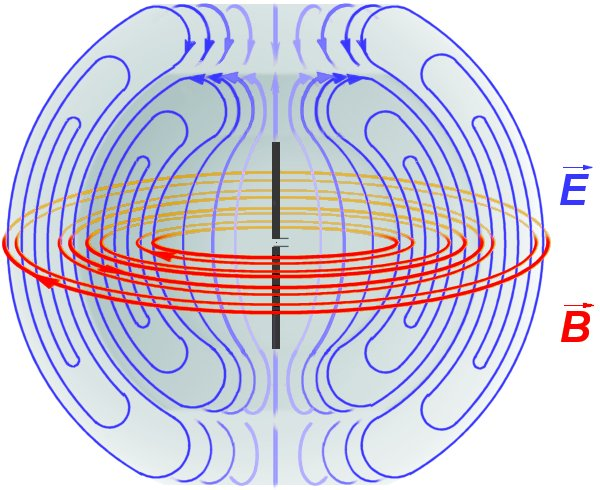
\includegraphics[width = 2.3cm]{./img/dipol_field.jpg}}
	\\
	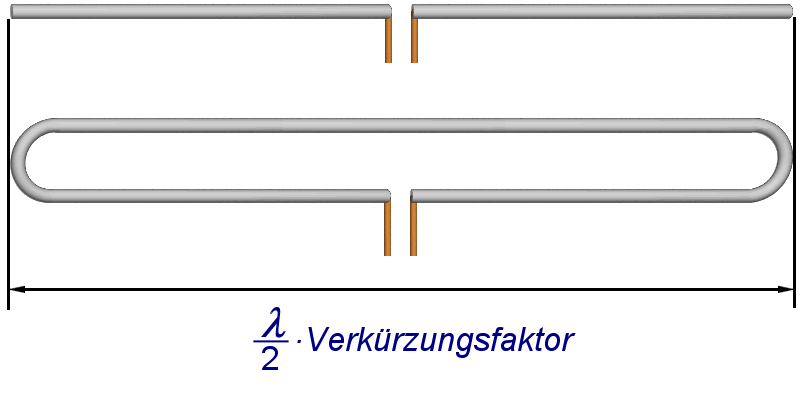
\includegraphics[width = 1cm]{./img/dipol_antenna.png} \quad 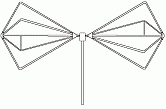
\includegraphics[width = 1cm]{./img/biconical_antenna.png} \quad 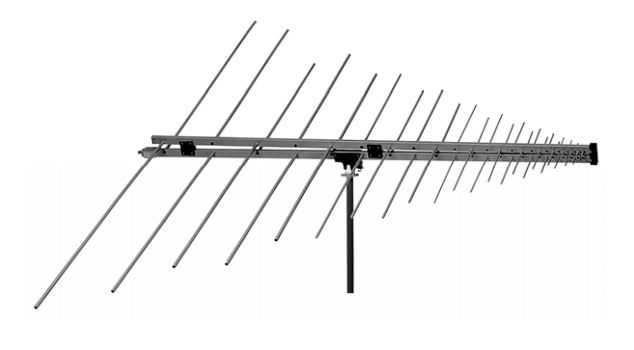
\includegraphics[width = 1.4cm]{./img/log-periodic_antenna.jpg} \quad 
	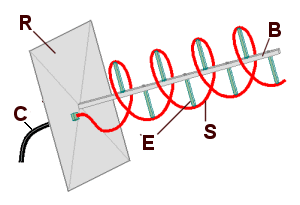
\includegraphics[width = 1.1cm]{./img/helical_antenna.png} \quad 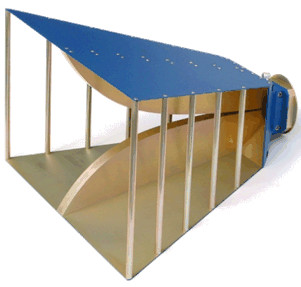
\includegraphics[width = 1cm]{./img/horn_antenna.jpg}
	
}	




\sectionbox{
	\subsection{GTEM Zelle}
	Störfestigkeitsmessung mit Transversalwelle mit $\cx Z = \cx Z_0$\\
	TEM-Zelle: Parallelplattenleitung, dazwischen kleines Objekt\\
	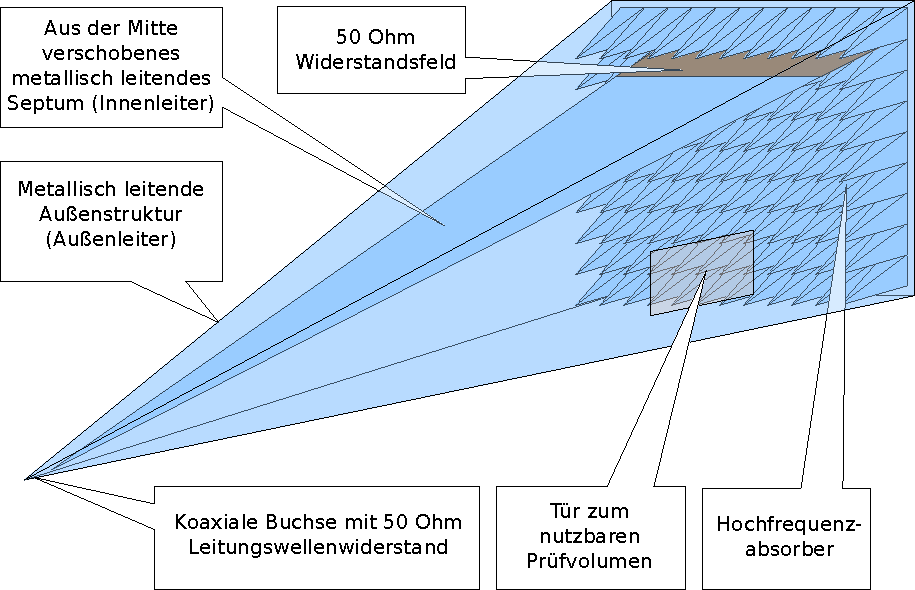
\includegraphics[width = \columnwidth]{./img/GTEM.pdf}
}

\sectionbox{
	\subsection{Freifeldmessung}
	\parbox{3.5cm}{Wenn zu messende Objekte zu groß für die Messkammer ist.\\
	Freie Ellipse: Reflektierte Wellen müssen mindestens doppelten Weg zurücklegen. Messequipment muss geschirmt werden.\\
	Probleme: Wetter, Bodenunebenheit, Rohre im Boden, Mobilfunk}\quad
	\parbox{3cm}{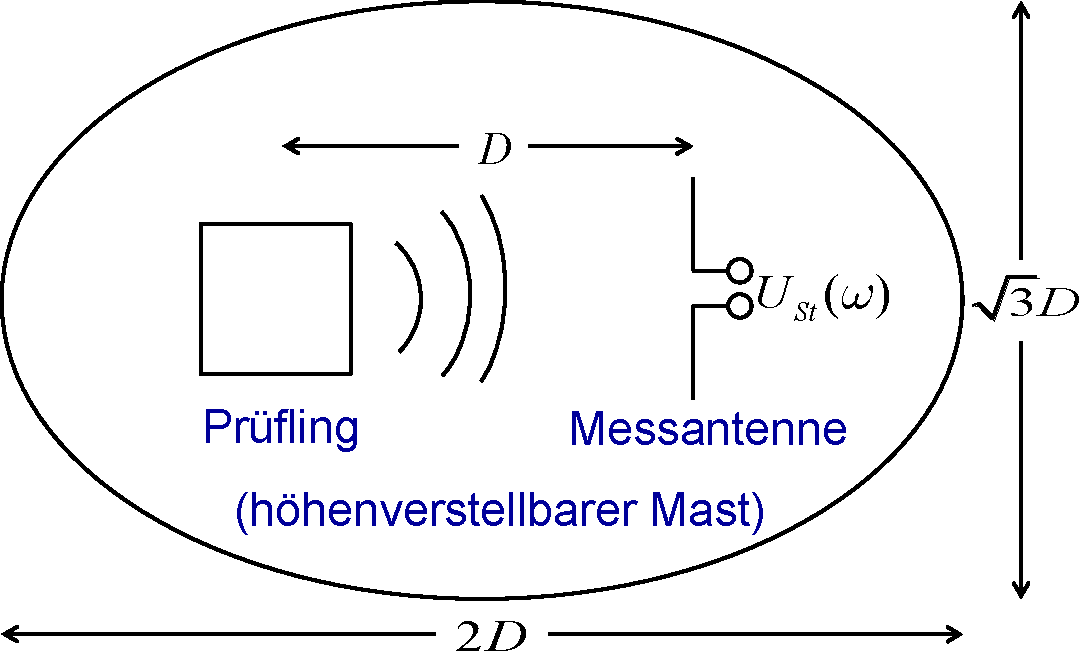
\includegraphics[width = 3cm]{./img/freifeld.pdf}}
}	


\sectionbox{
	\subsection{EMI Messung}
	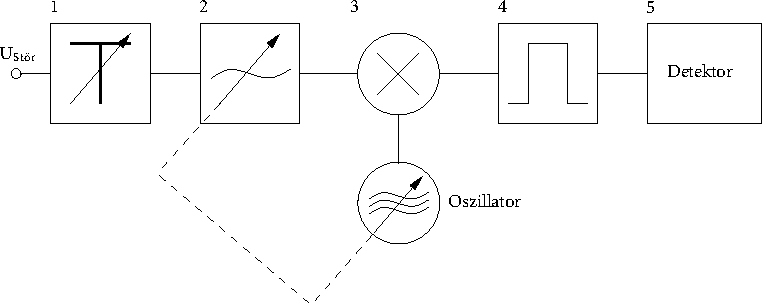
\includegraphics[width = 6cm]{./img/EMI.pdf}
}


% SECTION ====================================================================================
\section{Modellierung}
% ============================================================================================
\sectionbox{
	\textbf{Vorgehen:}\\
	Design Rule Checkers (z.B. EMBoardCheck von SimLab)
	Analytische Modellierung (einfache Strukturen)
	Leitungsmodellierung (CableMod von SimLab)
	Schaltungs-,Systemmodellierung (allgemein, z.B. Pspice)

	\textbf{Physikalische Berechnung:} FDTD, FEM, MOM, BEM, TLM\\
	Hybride Methoden:\\
	Berechnung der Leitungsparameter numerisch (FEM)\\
	Ausbreitung auf Mehrleitersystem (Leitungsgleichung)\\
	Berechnung der Abstrahlung mit Kabel als Quelle (Integralgleichungsmethode)\\
	Wichtig: Be critical to model and tool!\\
}

% SECTION ====================================================================================
\section{Maßnahmen gegen EMB (Beeinflussung)}
% ============================================================================================

\sectionbox{
	\subsection{Schirmung}
	Schirmungsfaktor $Q(\omega) = \frac{\vec H_{\ir innen}}{\vec H_{\ir ohne}}$\\

	\begin{description}
		\item[E-Dipol] (Nahfeld, hochohmig): Dämpfung nimmt mit zunehmender Frequenz ab, niedrige Frequenz $\ra$ Reflexion, hohe Frequenz $\ra$ Absorption, Abschirmung leicht realisierbar (dünnes Metall $\ra$ Skintiefe)
		\item[H-Dipol] (Nahfeld, niederohmig) Dämpfung nimmt mit steigender Frequenz zu, hauptsächlich Absorption, Abschirmung niederohmiger Magnetfelder bei niedrigen Frequenzen schwierig
		\item[EM Welle] (Fernfeld)Dämpfung in weitem Frequenzbereich frequenzunabhängig, unabhängig vom Abstand, Schirmung leicht
	\end{description}
}
\sectionbox{
	\subsection{Blitzschutz}
	Fanganordnungen sollen den Blitz einfangen\\
	Blitzableiter sollen den Strom abtransportieren\\
	Bestimmung der Orte mit Blitzkugelmethode\\
	Schutzerde: Evtl. Multiground (Achtung Erdschleifen!)\\
	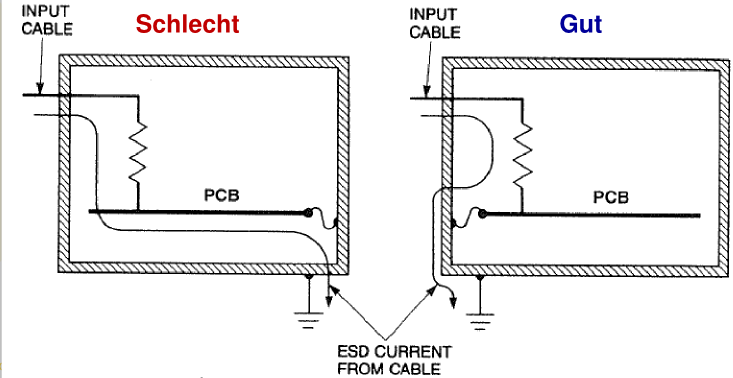
\includegraphics[width = 5cm]{./img/erdung.png}\\
	Schaltung sollte mind. 1 cm von nicht geerdeten Teilen und mind. 1 mm von geerdeten Gehäuseteilen entfernt sein!
}

	\subsection{PCB Design}


% SECTION ====================================================================================
\section{EMVU – Umweltverträglichkeit}
% ============================================================================================

\sectionbox{
	Effekte von el. mag. Feldern auf biologisches Material.
	\begin{description}
		\item[Thermische Effekte:] Erwärmung $P_A = \pi f \varepsilon_0 \iiint_V \varepsilon_r'' \norm{\vec E}^2 \diff v$\\
			Mikrowellenhören
		\item[Nicht-thermische Effekte]:\\ 
			auf Zellmembranen (Potential, Ströme, Ca$^{2+}$ Fluss)\\
			Nervensystem (EEG, Schlaf, Melatonin)\\
			Immunsystem, Krebsgefahr
		\item[Physikalische Primäreffekte:] Ladungsinfluenz, Feldeinkopplung, Ladungsbewegung, Polarisation von Molekülen
		\item[Biologische Sekundäreffekte:] Durch Primäreffekte ausgelöste biologische Effekte (Herzkammerflimmern, Verbrennungen)
	\end{description}

	Ab $\SI{5}{\giga \hertz}$ absorbiert nur obere Haut und Fettschicht\\
	Specific Absorbtion Rate: $\mathrm{SAR} = c \frac{\diff T}{\diff t}$\\

	\begin{tabular}{ll}
		Wissenschaftlich Effekte* & $\mathrm{SAR} = \SI{4}{\watt \per \kilogram}$\\
		Arbeiter & $\mathrm{SAR} = \SI{0.4}{\watt \per \kilogram}$\\
		Bevökerung & $\mathrm{SAR} = \SI{0.08}{\watt \per \kilogram}$\\
	\end{tabular}

	*: Erhöhung der Körpertemperatur um $\SI{1}{\celsius}$ nach 30 Minuten.\\
}


% SECTION ====================================================================================
\section{Übungen}
% ============================================================================================
Freileiter Bündelanordnung: Schwächeres Feld\\
Schmalbanige Störungen: Mikrowelle, Computer, Radio\\
Breitbandige Störung: Blitz, Relais, Schalter\\
\\
Relai Schalten: Hohe Induktion in der Spule (Maß: Diode)\\
Antennenstörung: Abstand, Abschirmung, Drehen der Antenne\\
EMI besser als Spektrumanalysator: Dynamik, Präzision, SNR\\
Aber SA schneller als EMI\\
EMI-Zeiten: Sweepzeit, Haltezeit, Gesamtzeit = SZ + HZ\\
\\
Antennenfaktor: $\frac{\norm{\vec E}}{U}$\\
EMS heißt elektromagnetische Störfestigkeit, Funktioniert Gerät\\
\\
Genzwerte: Physikalisch 1, Arbeiter $\frac{1}{10}$, Allgemein $\frac{1}{50}$\\
Keine Ecken, Schleifen, lange dünne Drähte in PCBs



% SECTION ====================================================================================
\section{Klausurfragen:}
% ============================================================================================
Wer gibt Normen vor?\\
Wo werden solche NOrmen produziert: Regierungen, Fabrikanten wegen Qualität, Militärische Standards (Robustheit)\\
Was wird Standardisiert? Prüfverfahren und Grenzwerte\\
Störquellen: Breibandige, Schmalbandig, Natürlich (Blitze, Entladungen) Stromerhöhung, 
Menschliche, Inustrielle Quellen (Schalter über Leitungen, Ladungstrennung durch Reibung)\\

Kopplungen: Leitungen oder Freiraum\\
Welle größer als Objekt: Statisch, getrennte Betrachtung von el. und mag. Wellen\\
Welle in der selben Größenordung: Gekoppelte Welleneffekte\\

Schirmung: Box (Achten auf Löcher in Wellenlängengrößenordnung), Materialen mit hohem $\mu_r$
Parallele Leitungen verhindern. Drähte verdrillen, Absorber dazwischen

Messkammer: Homogene Feldverteilung, Leistung aufdrehen\\
Messequipment: ANtennen, Filter, Reflektoren\\
Modellierung und Simmulation\\

EMVU: thermische (primär und sekundäreffekte) und nicht thermische\\
Immer 2 Gruppen testen.

% 01.08.13		10:30
% Nebenraum: Offene Tür, 30 min vorgesehen, davon ca. 20 min

% Ende der Spalten
\end{multicols*}

% Dokumentende
% ======================================================================
\end{document}

% ToDos:

